\hfill\\
\section{Hogwild Attention}\hfill

This section describes how to predict the Efrac and Mfrac of a jet using a stack of Transformer Encoders using Multi-Head Attention layers in the context of an event using track features and jet features as input.

\subsection{Model Input}\hfill

The model takes an entire event as an input. An event can be described as three tensors: jet tensor, jet-track tensor, and all-track tensor. Jet tensor $\mathbb{J}\in \mathbb{R}^{N_{jets} \times F_{jets}}$ has shape N jets per event with F input features, $p_T, \eta, \phi, m$. Jet-Track tensor $\mathbb{T}_{jet}\in \mathbb{R}^{N_{jets} \times N_{trks} \times F_{trks}}$ has shape number of jets per event, number of tracks per jet, and number of features per track, $p_T, \eta, \phi, q, d_0, z_0$. Lastly, All-Track tensor $\mathbb{T}_{Event}\in \mathbb{R}^{\times N_{trks} \times F_{trks}}$ has shape number of tracks per event and features per track. Each of these tensors if first passed through a linear preprocessing layer to transform them into the embedding space.

\subsection{Encoders Architecture}\hfill

Four transformer encoder stacks are used to enrich each tensor -- $\mathbb{J},\mathbb{T}_{jet},\mathbb{T}_{jet}$ -- with context from the event. Each encoder follows the NormFormer [*] architecture by (... et al). NormFormers conist of LayerNorms, LN(), multi-head attention, MHA(), skip connections, + operator, feed-forward network, FFN, which consists of a linear layer and a GELU activation function. These layers are the components of each encoder block.

First, each jet is enriched with associated tracks. Since each jet only carries four features, $p_T, \eta, \phi, m$, tracks within a radius of $\Delta R = 0.4$ are used in the first encoder stack to achieve a rich representation of each jet.

\begin{align}
    \mathbb{T}_{context} &= \mathbb{T}_{jet} + LN(MHA(LN(\mathbb{T}_{jet}), LN(\mathbb{T}_{jet}), LN(\mathbb{T}_{jet}))) \\
    \mathbb{T}_{embed} &= \mathbb{T}_{context} + FFN (\mathbb{T}_{context}) \\
    \mathbb{T}_{aggregated} &= \sum_{dim=1} \mathbb{T}_{embed} \\ 
    \mathbb{J}_{enriched} &= FFN(\mathbb{J} \mathop{\oplus}_{dim=1} \mathbb{T}_{aggregated})
\end{align}
$\mathbb{T}_{jet}$, $\mathbb{T}_{context}$, and $\mathbb{T}_{embed}$ all have shape $N_{jet} \times N_{trk} \times E_{dim}$. Then the summation operator reduces the $N_{trk}$ dimension which will then match the dimension of $\mathbb{J}$ with shape $N_{jet} \times E_{dim}$. The jet and aggregated track tensors are concatenated along the embedding dimension, and the FFN has input $N_{jet} \times 2\cdot E_{dim}$ and outputs $\mathbb{J}$ of shape $N_{jet} \times E_{dim}$. This encoder block can be interpreted physically as learning to enrich the jet in the context of associated particles. For example, if there is are particles that resemble b-hadron decay, this encoder block might enrich this jet as a b-jet in the latent space.

Second, $\mathbb{T}_{event}$ with shape $N_{trk} \times E_{dim}$ are enriched using an encoder block using self-attention:
\begin{align}
    \mathbb{T}_{context} &= \mathbb{T}_{event} + LN(MHA(LN(\mathbb{T}_{event}), LN(\mathbb{T}_{event}), LN(\mathbb{T}_{event}))) \\
    \mathbb{T}_{embed} &= \mathbb{T}_{context} + FFN (\mathbb{T}_{context}) \\
\end{align}
The purpose of this encoder is to update all tracks in the context of the event and initialize them for cross attention with jets.

Third, cross attention between $\mathbb{J}_{enriched}$ and $\mathbb{T}_{embed}$ is performed to update the jets in the context of all tracks of the event.

\begin{align}
    \mathbb{J}_{context} &= \mathbb{J}_{enriched} + LN(MHA(LN(\mathbb{J}_{enriched}), LN(\mathbb{T}_{event}), LN(\mathbb{T}_{event}))) \\
    \mathbb{J}_{embed} &= \mathbb{J}_{context} + FFN (\mathbb{J}_{context}) \\
\end{align}

This encoder allows tracks to update the jet embedding in the context of an event. For example, if we consier $t \rightarrow Wb \rightarrow l\nu b$, this encoder allows the high energy lepton, l, to update the context of the b-jet.

Fourth and finally, $\mathbb{J}_{embed}$ with shape $N_{jet} \times E_{dim}$ is enriched using a encoder block using self attention:

\begin{align}
    \mathbb{J}_{context} &= \mathbb{J}_{embed} + LN(MHA(LN(\mathbb{J}_{embed}), LN(\mathbb{J}_{embed}), LN(\mathbb{J}_{embed}))) \\
    \mathbb{J}_{embed} &= \mathbb{J}_{context} + FFN (\mathbb{J}_{context}) \\
\end{align}

This encoder is performed last because at this stage the jets have achieved a rich representation after passing through the previous encoders. This last encoder allows jets to update their representation in the context of an event. This encoder can be interpreted physically as allowing jets to update representations according to conservation of momentum or other properties that might be shared between jets.

Lastly, the embedded jet vectors are passed through a final classification layer to predict the continuous pileup fraction label.

\subsection{Results}\hfill

The model was constructed using a stack of 3x jet associated-track encoders, 3x all track encoders, 3x jet all track encoders, and finally 3x jet encoders. In total the model has 4.1M parameters and took about 1 hour to converge on an NVIDIA 3090 using a sample size of 10k $t\bar{t}$ events with around 500k jets and 10M charged tracks greater than 400 MeV.

\begin{figure}[h!]
\centering
\begin{subfigure}{.25\textwidth}
  \centering
  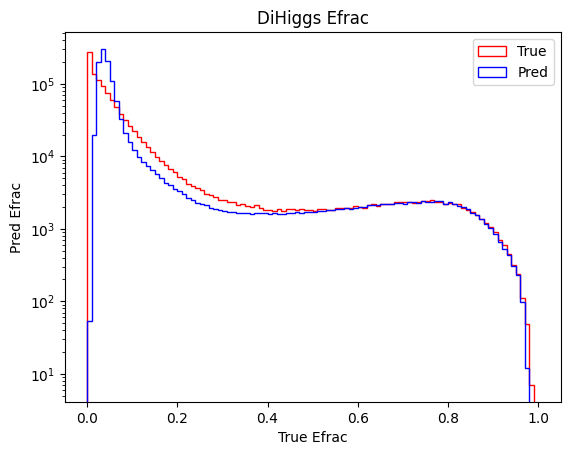
\includegraphics[width=1\linewidth]{diHiggs_Efrac_1d.png}
  \caption{}
  \label{fig:sub1}
\end{subfigure}%
\begin{subfigure}{.25\textwidth}
  \centering
  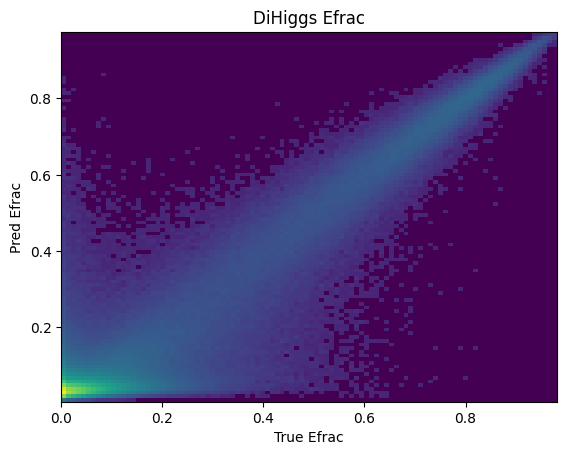
\includegraphics[width=1\linewidth]{diHiggs_Efrac_2d.png}
  \caption{}
  \label{fig:sub2}
\end{subfigure}
\begin{subfigure}{.25\textwidth}
  \centering
  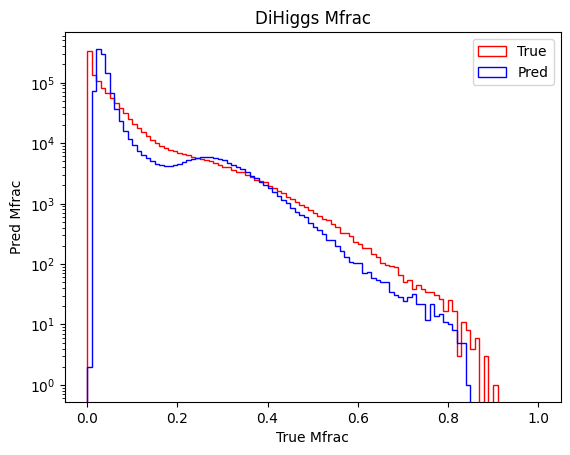
\includegraphics[width=1\linewidth]{diHiggs_Mfrac_1d.png}
  \caption{}
  \label{fig:sub1}
\end{subfigure}%
\begin{subfigure}{.25\textwidth}
  \centering
  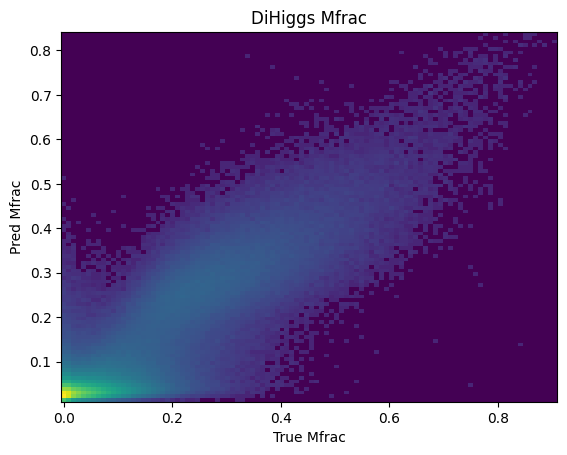
\includegraphics[width=1\linewidth]{diHiggs_Mfrac_2d.png}
  \caption{}
  \label{fig:sub2}
\end{subfigure}
\caption{The predicted Mass fraction of jets. Figure (a) 1-D Histogram. Figure (b) 2-D Historgram.}
\label{fig:test}
\end{figure}

\begin{figure}[h!]
\centering
\begin{subfigure}{.45\textwidth}
  \centering
  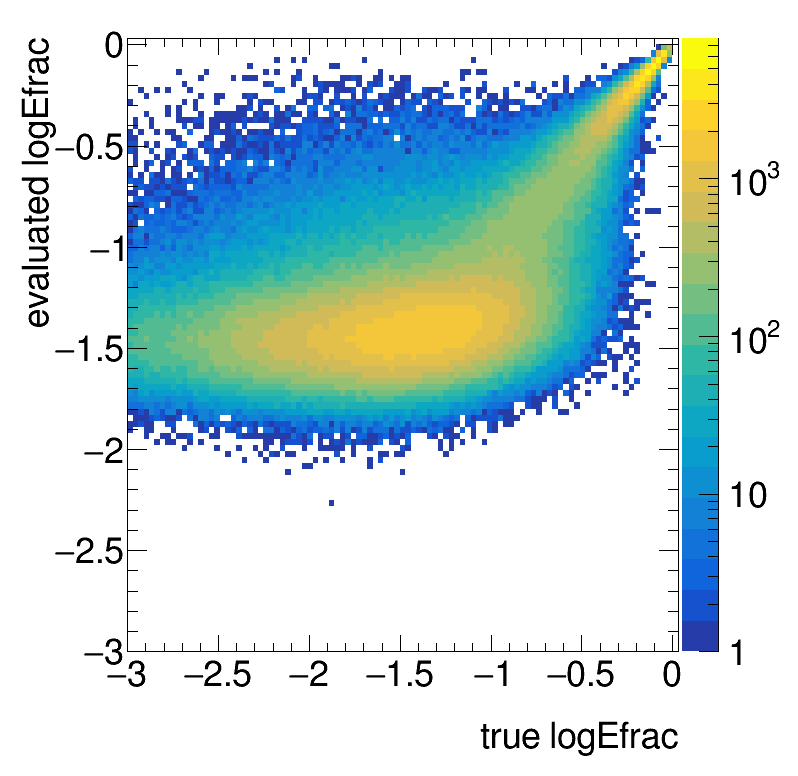
\includegraphics[width=1\linewidth]{logEfrac_eval_vs_true_HH_mu60_20k.png}
  \caption{}
  \label{fig:sub1}
\end{subfigure}%
\begin{subfigure}{.45\textwidth}
  \centering
  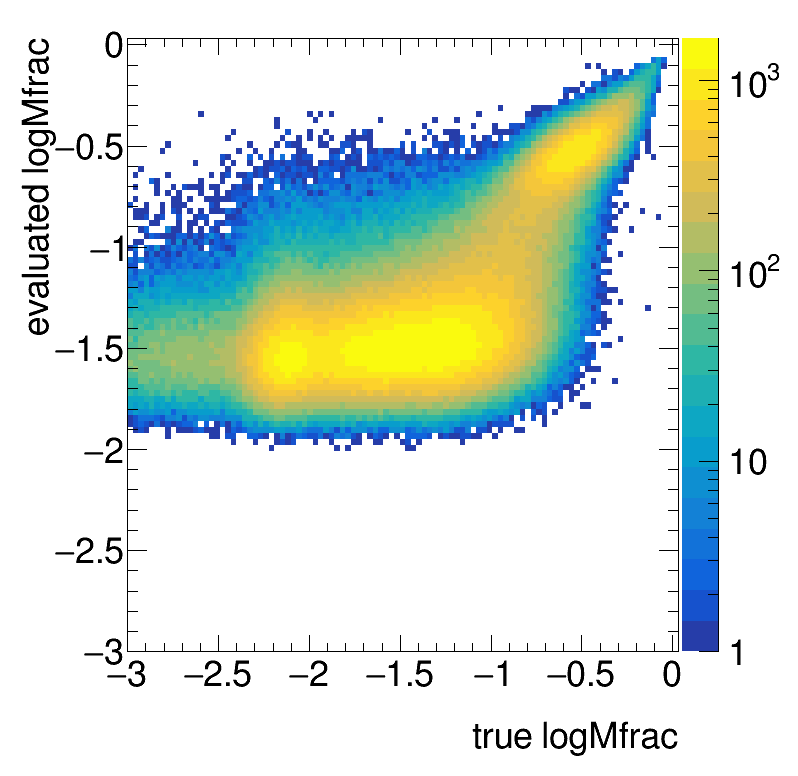
\includegraphics[width=1\linewidth]{logMfrac_eval_vs_true_HH_mu60_20k.png}
  \caption{}
  \label{fig:sub2}
\end{subfigure}
\caption{The predicted fractions vs the true fraction on a log scale. Figure (a) Efrac. Figure (b) Mfrac.}
\label{fig:test}
\end{figure}

\begin{center}
\begin{tabular}{||c c ||} 
 \hline
 Metric & Value  \\ [0.5ex] 
 \hline\hline
 Train Loss & 0.0016  \\ 
 \hline
 Val Loss & 0.0018 \\
 \hline
 Test Loss & 0.0022\\
 \hline
 Test MAE & 0.017 \\
 \hline
 Test RMSE & 0.046 \\ [1ex] 
 \hline
\end{tabular}
\end{center}

The model is trained using mean squared error loss. After converging, the train loss reaches around 0.00164, validation loss of about 0.0018, and train loss of 0.0022. The mean absolute error, MAE, of about 0.017, and the root mean squared error, RMSE, of about 0.046.

